% Tema 11. Conversión de T11-CURVAS PARAM.pptx: 58 diapositivas.
% Compilar desde la raíz: pdflatex -interaction=nonstopmode temas/tema11.tex
\documentclass[main.tex]{subfiles}

\begin{document}
\graphicspath{{imagenes/tema11/}{../imagenes/tema11/}}

% Diapositiva 1
\portadatema{11}{Curvas paramétricas}

% Diapositiva 2
\begin{frame}[t]{Introducción}
Hasta ahora se han utilizado dos formas de representar curvas en el plano:\begin{itemize}
\item Explícita: $y=f(x)$. Por ejemplo, $y=ax^2+bx+c$.
\item Implícita: $f(x,y)=0$. Por ejemplo, $x^2+y^2-r^2=0$.
\end{itemize}\begin{columns}[T]\begin{column}{.48\textwidth}\figura{r2_rId2.png}{.9}{.35}\end{column}\begin{column}{.48\textwidth}\figura{r2_rId3.png}{.8}{.35}\end{column}\end{columns}Una curva implícita no siempre es la gráfica de una función $y=f(x)$.
\end{frame}

% Diapositiva 3
\begin{frame}[t]{Introducción}
¿Cómo se pueden modelar curvas reales?\par\medskip Por ejemplo, las curvas que rigen el movimiento de una animación.\begin{columns}[T]\begin{column}{.48\textwidth}\figura{r3_rId4.png}{1}{.42}\end{column}\begin{column}{.48\textwidth}\figura{r3_rId5.png}{.9}{.42}\end{column}\end{columns}\begin{center}\large Hay que utilizar un nuevo enfoque.\end{center}
\end{frame}

% Diapositiva 4
\begin{frame}[t]{Introducción}
Consiste en expresar la relación entre $x$ e $y$ de la forma\[x=f_1(t),\qquad y=f_2(t).\]Donde $f_1$ y $f_2$ son funciones del parámetro $t$.\par\bigskip Los valores de $x$ e $y$ se expresan en términos de una variable independiente, denominada \textbf{parámetro}, que generalmente se elige entre $0$ y $1$.
\end{frame}

% Diapositiva 5
\begin{frame}[t]{Introducción}
Si se tiene una serie finita de puntos\[(x_0,y_0),\ldots,(x_n,y_n),\]y se quiere aproximar una curva que pase por todos ellos, se busca\[x(t_i)=x_i,\qquad y(t_i)=y_i,\qquad i=0,\ldots,n.\]El parámetro se elige de modo que $t_0$ corresponda al primer punto $(x_0,y_0)$ y $t_n$ al último $(x_n,y_n)$.
\end{frame}

% Diapositiva 6
\begin{frame}[t]{Introducción}
De esta forma se tiene una aplicación\[\mathbf r:[0,1]\longrightarrow\mathbb R^2,\qquad t\longmapsto (x(t),y(t)).\]\figura{r6_rId3.png}{.9}{.2}Se pueden ver como dos funciones combinadas:\begin{center}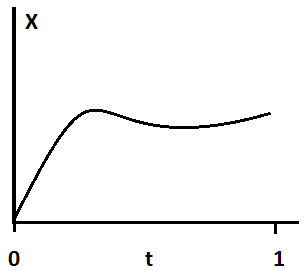
\includegraphics[width=.29\textwidth,height=.3\textheight,keepaspectratio]{r6_rId4.png}\hfill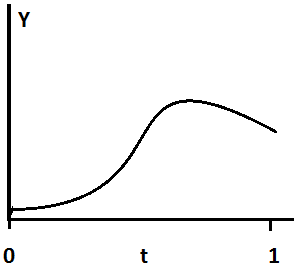
\includegraphics[width=.29\textwidth,height=.3\textheight,keepaspectratio]{r6_rId5.png}\hfill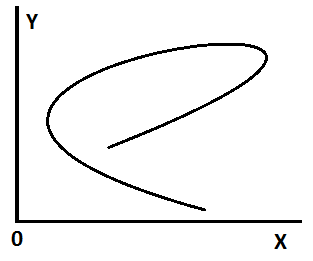
\includegraphics[width=.29\textwidth,height=.3\textheight,keepaspectratio]{r6_rId6.png}\hfill\end{center}
\end{frame}

% Diapositiva 7
\begin{frame}[t]{Introducción}
Se suelen utilizar funciones que son polinomios en un parámetro $t$.\begin{itemize}
\item Eficiencia en el cómputo: operaciones elementales, como sumas y multiplicaciones.
\item Fáciles de derivar e integrar.
\item Permiten aproximar funciones continuas con tanta precisión como se quiera (teorema de aproximación de Weierstrass).
\item Ofrecen control local utilizando funciones definidas a trozos.
\end{itemize}Se asume que $t$ varía entre $0$ y $1$.
\end{frame}

% Diapositiva 8
\begin{frame}[t]{Ejemplo de interpolación}
Se desea construir un par de polinomios de Lagrange para aproximar la siguiente curva, usando los puntos de muestreo indicados.\figura{r8_rId2.png}{.65}{.58}
\end{frame}

% Diapositiva 9
\begin{frame}[t]{Ejemplo de interpolación}
Se eligen los puntos $t_i$ equidistantes en $[0,1]$, obteniendo los siguientes datos:\begingroup\small\setlength{\tabcolsep}{2pt}\begin{center}\begin{tabular}{|C{.14\textwidth}|C{.14\textwidth}|C{.14\textwidth}|C{.14\textwidth}|C{.14\textwidth}|C{.14\textwidth}|}\hline
$i$ & $0$ & $1$ & $2$ & $3$ & $4$\\\hline
\rule[-1.5mm]{0pt}{5mm}$t_i$ & 0 & $\frac14$ & $\frac12$ & $\frac34$ & 1\\\hline
\rule[-1.5mm]{0pt}{5mm}$x_i$ & -1 & 0 & 1 & 0 & 1\\\hline
\rule[-1.5mm]{0pt}{5mm}$y_i$ & 0 & 1 & $\frac12$ & 0 & -1\\\hline
\end{tabular}\end{center}\endgroup\figura{r9_rId4.png}{.55}{.4}
\end{frame}

% Diapositiva 10
\begin{frame}[t]{Ejemplo de interpolación}
Con los pares $(t_i,x_i)$ se obtiene el polinomio de Lagrange\[x(t)=\left(\left(\left(64t-\frac{352}{3}\right)t+60\right)t-\frac{14}{3}\right)t-1.\]\medskip Con los pares $(t_i,y_i)$ se obtiene\[y(t)=\left(\left(\left(-\frac{64}{3}t+48\right)t-\frac{116}{3}\right)t+11\right)t.\]
\end{frame}

% Diapositiva 11
\begin{frame}[t]{Ejemplo de interpolación}
Representando este sistema paramétrico, se obtiene la curva:\figura{r11_rId2.png}{.7}{.58}A pesar de pasar por los puntos de muestreo, es una aproximación relativamente imprecisa.
\end{frame}

% Diapositiva 12
\begin{frame}[t]{Objetivo del tema}
\vfill\begin{center}\Large\textbf{Objetivo}\par\bigskip Construir curvas de una manera fácil y exacta.\par\bigskip\textbf{¿Cómo?}\end{center}\vfill
\end{frame}

% Diapositiva 13
\begin{frame}[t]{Curvas de Bézier}
Las curvas de Bézier se desarrollaron en la década de 1960 para el trazado de dibujos técnicos en el diseño aeronáutico y de automóviles.\par\medskip Anteriormente, las curvas se trazaban por medio de reglas francesas.\figura{r13_rId2.png}{.65}{.5}
\end{frame}

% Diapositiva 14
\begin{frame}[t]{Curvas de Bézier}
En 1959, Paul de Casteljau (Citroën) ideó una formulación matemática para diseñar las formas curvas de los coches.\par\medskip En la década de 1960, Pierre Bézier (Renault) desarrolló de forma independiente otra formulación matemática.\begin{columns}[T]\begin{column}{.48\textwidth}\figura{r14_rId2.png}{1}{.38}\end{column}\begin{column}{.48\textwidth}\figura{r14_rId3.png}{1}{.38}\end{column}\end{columns}
\end{frame}

% Diapositiva 15
\begin{frame}[t]{Curvas de Bézier}
\begin{itemize}
\item Se definen por una serie de puntos de control.
\item La curva empieza en el primer punto de control y termina en el último.
\item Los puntos intermedios atraen hacia sí la curva.
\end{itemize}\figura{r15_rId3.png}{.7}{.48}\[t\in[0,1].\]
\end{frame}

% Diapositiva 16
\begin{frame}[t]{Curvas de Bézier lineales}
Con dos puntos de control $P_0$ y $P_1$ se obtiene un segmento:\[\mathbf b(t)=(1-t)P_0+tP_1,\qquad 0\leq t\leq1.\]\figura{r16_rId3.png}{.85}{.5}
\end{frame}

% Diapositiva 17
\begin{frame}[t]{Curvas de Bézier cuadráticas}
Con tres puntos de control $P_0,P_1,P_2$, se construyen\[C(t)=(1-t)P_0+tP_1,\qquad D(t)=(1-t)P_1+tP_2.\]Interpolando entre ambos:\[\begin{aligned}\mathbf b(t)&=(1-t)C(t)+tD(t)\\&=(1-t)^2P_0+2t(1-t)P_1+t^2P_2.\end{aligned}\]\figura{r17_rId3.png}{.65}{.33}
\end{frame}

% Diapositiva 18
\begin{frame}[t]{Curvas de Bézier cúbicas}
\small Con cuatro puntos de control $P_0,P_1,P_2,P_3$:\[\begin{aligned}C&=(1-t)P_0+tP_1, &D&=(1-t)P_1+tP_2,\\ E&=(1-t)P_2+tP_3, &F&=(1-t)C+tD,\\ G&=(1-t)D+tE, &\mathbf b&=(1-t)F+tG.\end{aligned}\]\[\mathbf b(t)=(1-t)^3P_0+3t(1-t)^2P_1+3t^2(1-t)P_2+t^3P_3.\]\figura{r18_rId3.png}{.85}{.34}
\end{frame}

% Diapositiva 19
\begin{frame}[t]{Curvas de Bézier de grado superior}
De esta forma se pueden generar curvas de cualquier grado.\figura{r19_rId2.png}{.9}{.7}
\end{frame}

% Diapositiva 20
\begin{frame}[t]{Polígonos de Bézier}
Los puntos de control de una curva de Bézier forman el \textbf{polígono de Bézier}.\begin{center}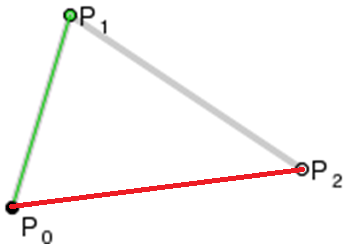
\includegraphics[width=.3\textwidth,height=.55\textheight,keepaspectratio]{r20_rId2.png}\hfill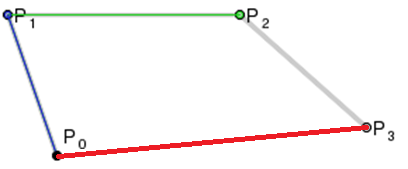
\includegraphics[width=.3\textwidth,height=.55\textheight,keepaspectratio]{r20_rId3.png}\hfill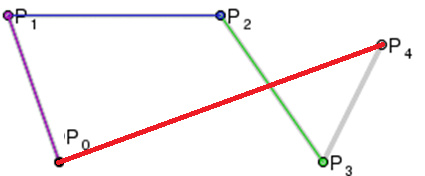
\includegraphics[width=.3\textwidth,height=.55\textheight,keepaspectratio]{r20_rId4.png}\hfill\end{center}
\end{frame}

% Diapositiva 21
\begin{frame}[t]{Curvas de Bézier: formalización}
\begin{itemize}
\item Forma explícita: polinomios de Bernstein.
\item Algoritmo de de Casteljau.
\item Forma matricial: curvas de Bézier cúbicas.
\end{itemize}
\end{frame}

% Diapositiva 22
\begin{frame}[t]{Polinomios de Bernstein}
Se parte de la expresión\[(t+(1-t))^n=1.\]Aplicando el binomio de Newton:\[1=\sum_{i=0}^{n}\binom ni t^i(1-t)^{n-i}.\]Se denominan \textbf{polinomios de Bernstein de grado $n$}\[\boxed{B_i^n(t)=\binom ni t^i(1-t)^{n-i}},\qquad i=0,\ldots,n.\]
\end{frame}

% Diapositiva 23
\begin{frame}[t]{Polinomios de Bernstein: ejemplo}
Polinomios de Bernstein de grado 1:\[\begin{aligned}B_0^1(t)&=\binom{1}{0}t^{0}(1-t)^{1}=1-t\\[3mm]B_1^1(t)&=\binom{1}{1}t^{1}(1-t)^{0}=t\end{aligned}\]
\end{frame}

% Diapositiva 24
\begin{frame}[t]{Polinomios de Bernstein: ejemplo}
Polinomios de Bernstein de grado 2:\[\begin{aligned}B_0^2(t)&=\binom{2}{0}t^{0}(1-t)^{2}=(1-t)^2\\[3mm]B_1^2(t)&=\binom{2}{1}t^{1}(1-t)^{1}=2t(1-t)\\[3mm]B_2^2(t)&=\binom{2}{2}t^{2}(1-t)^{0}=t^2\end{aligned}\]
\end{frame}

% Diapositiva 25
\begin{frame}[t]{Polinomios de Bernstein: ejemplo}
Polinomios de Bernstein de grado 3:\[\begin{aligned}B_0^3(t)&=\binom{3}{0}t^{0}(1-t)^{3}=(1-t)^3\\[3mm]B_1^3(t)&=\binom{3}{1}t^{1}(1-t)^{2}=3t(1-t)^2\\[3mm]B_2^3(t)&=\binom{3}{2}t^{2}(1-t)^{1}=3t^2(1-t)\\[3mm]B_3^3(t)&=\binom{3}{3}t^{3}(1-t)^{0}=t^3\end{aligned}\]
\end{frame}

% Diapositiva 26
\begin{frame}[t]{Bernstein: propiedades}
\begin{columns}[T]\begin{column}{.48\textwidth}\textbf{Grado 1}\begingroup\scriptsize\setlength{\tabcolsep}{2pt}\begin{center}\begin{tabular}{|C{.19\textwidth}|C{.19\textwidth}|C{.19\textwidth}|C{.19\textwidth}|}\hline
$t$ & $B_0^1$ & $B_1^1$ & Suma\\\hline
\rule[-1.5mm]{0pt}{3.7mm}0 & 1 & 0 & 1\\\hline
\rule[-1.5mm]{0pt}{3.7mm}0,2 & 0,8 & 0,2 & 1\\\hline
\rule[-1.5mm]{0pt}{3.7mm}0,4 & 0,6 & 0,4 & 1\\\hline
\rule[-1.5mm]{0pt}{3.7mm}0,6 & 0,4 & 0,6 & 1\\\hline
\rule[-1.5mm]{0pt}{3.7mm}0,8 & 0,2 & 0,8 & 1\\\hline
\rule[-1.5mm]{0pt}{3.7mm}1 & 0 & 1 & 1\\\hline
\end{tabular}\end{center}\endgroup\end{column}\begin{column}{.48\textwidth}\textbf{Grado 2}\begingroup\scriptsize\setlength{\tabcolsep}{2pt}\begin{center}\begin{tabular}{|C{.155\textwidth}|C{.155\textwidth}|C{.155\textwidth}|C{.155\textwidth}|C{.155\textwidth}|}\hline
$t$ & $B_0^2$ & $B_1^2$ & $B_2^2$ & Suma\\\hline
\rule[-1.5mm]{0pt}{3.7mm}0 & 1 & 0 & 0 & 1\\\hline
\rule[-1.5mm]{0pt}{3.7mm}0,2 & 0,64 & 0,32 & 0,04 & 1\\\hline
\rule[-1.5mm]{0pt}{3.7mm}0,4 & 0,36 & 0,48 & 0,16 & 1\\\hline
\rule[-1.5mm]{0pt}{3.7mm}0,6 & 0,16 & 0,48 & 0,36 & 1\\\hline
\rule[-1.5mm]{0pt}{3.7mm}0,8 & 0,04 & 0,32 & 0,64 & 1\\\hline
\rule[-1.5mm]{0pt}{3.7mm}1 & 0 & 0 & 1 & 1\\\hline
\end{tabular}\end{center}\endgroup\end{column}\end{columns}\textbf{Grado 3}\begingroup\scriptsize\setlength{\tabcolsep}{2pt}\begin{center}\begin{tabular}{|C{.14\textwidth}|C{.14\textwidth}|C{.14\textwidth}|C{.14\textwidth}|C{.14\textwidth}|C{.14\textwidth}|}\hline
$t$ & $B_0^3$ & $B_1^3$ & $B_2^3$ & $B_3^3$ & Suma\\\hline
\rule[-1.5mm]{0pt}{3.7mm}0 & 1 & 0 & 0 & 0 & 1\\\hline
\rule[-1.5mm]{0pt}{3.7mm}0,2 & 0,512 & 0,384 & 0,096 & 0,008 & 1\\\hline
\rule[-1.5mm]{0pt}{3.7mm}0,4 & 0,216 & 0,432 & 0,288 & 0,064 & 1\\\hline
\rule[-1.5mm]{0pt}{3.7mm}0,6 & 0,064 & 0,288 & 0,432 & 0,216 & 1\\\hline
\rule[-1.5mm]{0pt}{3.7mm}0,8 & 0,008 & 0,096 & 0,384 & 0,512 & 1\\\hline
\rule[-1.5mm]{0pt}{3.7mm}1 & 0 & 0 & 0 & 1 & 1\\\hline
\end{tabular}\end{center}\endgroup
\end{frame}

% Diapositiva 27
\begin{frame}[t]{Bernstein: propiedades}
La suma de todos los polinomios de Bernstein de un mismo grado es $1$, para cualquier valor de $t$:\[\sum_{i=0}^{n}B_i^n(t)=1.\]\figura{r27_rId5.png}{.75}{.56}
\end{frame}

% Diapositiva 28
\begin{frame}[t]{Bernstein: propiedades}
\small\begin{itemize}
\item Son linealmente independientes y forman una base de los polinomios de grado menor o igual que $n$.
\item Son simétricos: $B_i^n(t)=B_{n-i}^n(1-t)$.
\item Sus posibles raíces son $0$ y $1$: aparecen cuando el exponente correspondiente es positivo.
\item Son positivos en todo el intervalo $(0,1)$.
\item Satisfacen la relación de recurrencia\[B_i^n(t)=(1-t)B_i^{n-1}(t)+tB_{i-1}^{n-1}(t),\]tomando $B_i^{n-1}=0$ si el índice queda fuera del rango $0,\ldots,n-1$.
\end{itemize}
\end{frame}

% Diapositiva 29
\begin{frame}[t]{Curvas de Bézier con Bernstein}
\small Son curvas paramétricas en las que $t$ varía entre $0$ y $1$. Los polinomios de Bernstein ponderan los puntos de control: los pesos son no negativos y suman $1$.\par\medskip\scriptsize Grados 1, 2 y 3: pesos en porcentaje (redondeados).\begingroup\scriptsize\setlength{\tabcolsep}{2pt}\begin{center}\begin{tabular}{|C{.082\textwidth}|C{.082\textwidth}|C{.082\textwidth}|C{.082\textwidth}|C{.082\textwidth}|C{.082\textwidth}|C{.082\textwidth}|C{.082\textwidth}|C{.082\textwidth}|C{.082\textwidth}|}\hline
$t$ & $P_0$ & $P_1$ & $P_0$ & $P_1$ & $P_2$ & $P_0$ & $P_1$ & $P_2$ & $P_3$\\\hline
\rule[-1.5mm]{0pt}{5mm}0 & 100\% & 0\% & 100\% & 0\% & 0\% & 100\% & 0\% & 0\% & 0\%\\\hline
\rule[-1.5mm]{0pt}{5mm}0,2 & 80\% & 20\% & 64\% & 32\% & 4\% & 51\% & 38\% & 10\% & 1\%\\\hline
\rule[-1.5mm]{0pt}{5mm}0,4 & 60\% & 40\% & 36\% & 48\% & 16\% & 22\% & 43\% & 29\% & 6\%\\\hline
\rule[-1.5mm]{0pt}{5mm}0,6 & 40\% & 60\% & 16\% & 48\% & 36\% & 6\% & 29\% & 43\% & 22\%\\\hline
\rule[-1.5mm]{0pt}{5mm}0,8 & 20\% & 80\% & 4\% & 32\% & 64\% & 1\% & 10\% & 38\% & 51\%\\\hline
\rule[-1.5mm]{0pt}{5mm}1 & 0\% & 100\% & 0\% & 0\% & 100\% & 0\% & 0\% & 0\% & 100\%\\\hline
\end{tabular}\end{center}\endgroup\[\underbrace{B_0^1,B_1^1}_{\text{grado 1}}\qquad\underbrace{B_0^2,B_1^2,B_2^2}_{\text{grado 2}}\qquad\underbrace{B_0^3,B_1^3,B_2^3,B_3^3}_{\text{grado 3}}\]
\end{frame}

% Diapositiva 30
\begin{frame}[t]{Curvas de Bézier con Bernstein}
\vspace{8mm}\[\boxed{\mathbf b(t)=(x(t),y(t))=\sum_{i=0}^{n}B_i^n(t)P_i},\qquad t\in[0,1].\]\bigskip Donde los $P_i$ son los puntos de control o vértices del polígono de Bézier.
\end{frame}

% Diapositiva 31
\begin{frame}[t]{Curvas de Bézier: ejemplo}
\small Para $P_0=(1,1)$, $P_1=(2,5)$ y $P_2=(6,3)$:\[\mathbf b(t)=(1-t)^2(1,1)+2t(1-t)(2,5)+t^2(6,3).\]\[x(t)=3t^2+2t+1,\qquad y(t)=-6t^2+8t+1.\]\figura{r31_rId4.png}{.7}{.48}
\end{frame}

% Diapositiva 32
\begin{frame}[t]{Curvas de Bézier: recursividad}
Aprovechando la recurrencia de los polinomios de Bernstein, se obtiene la \textbf{formulación de de Casteljau}.\par\medskip La curva de Bézier de grado menor o igual que $n$ es\[\mathbf b(t)=\mathbf b_0^n(t),\]donde\[\begin{aligned}\mathbf b_i^0(t)&=P_i, &&i=0,\ldots,n,\\\mathbf b_i^k(t)&=(1-t)\mathbf b_i^{k-1}(t)+t\mathbf b_{i+1}^{k-1}(t),\\ &&&k=1,\ldots,n,\quad i=0,\ldots,n-k.\end{aligned}\]
\end{frame}

% Diapositiva 33
\begin{frame}[t]{Formulación de de Casteljau}
\begin{minipage}[t]{\textwidth}\begin{center}\begin{tikzpicture}[x=2.5cm,y=.85cm,every node/.style={font=\small,minimum width=13mm,minimum height=6mm}]\path[use as bounding box](-.5,-3.6) rectangle (3.6,.5);\node (n00) at (0,0.0) {$P_0$};\node (n01) at (0,-1.0) {$P_1$};\node (n02) at (0,-2.0) {$P_2$};\node (n10) at (1,-0.5) {$\mathbf b_0^1$};\draw[->,gray] (n00) -- (n10);\draw[->,gray] (n01) -- (n10);\node (n11) at (1,-1.5) {$\mathbf b_1^1$};\draw[->,gray] (n01) -- (n11);\draw[->,gray] (n02) -- (n11);\node (n20) at (2,-1.0) {$\mathbf b_0^2$};\draw[->,gray] (n10) -- (n20);\draw[->,gray] (n11) -- (n20);\end{tikzpicture}\end{center}\end{minipage}\small\[\begin{aligned}\mathbf b_0^1&=(1-t)P_0+tP_1,&\mathbf b_1^1&=(1-t)P_1+tP_2,\\\mathbf b_0^2&=(1-t)\mathbf b_0^1+t\mathbf b_1^1\\&=(1-t)^2P_0+2t(1-t)P_1+t^2P_2.\end{aligned}\]
\end{frame}

% Diapositiva 34
\begin{frame}[t]{Formulación de de Casteljau}
\begin{minipage}[t]{\textwidth}\begin{center}\begin{tikzpicture}[x=2.5cm,y=.85cm,every node/.style={font=\small,minimum width=13mm,minimum height=6mm}]\path[use as bounding box](-.5,-3.6) rectangle (3.6,.5);\node (n00) at (0,0.0) {$P_0$};\node (n01) at (0,-1.0) {$P_1$};\node (n02) at (0,-2.0) {$P_2$};\node (n03) at (0,-3.0) {$P_3$};\node (n10) at (1,-0.5) {$\mathbf b_0^1$};\draw[->,gray] (n00) -- (n10);\draw[->,gray] (n01) -- (n10);\node (n11) at (1,-1.5) {$\mathbf b_1^1$};\draw[->,gray] (n01) -- (n11);\draw[->,gray] (n02) -- (n11);\node (n12) at (1,-2.5) {$\mathbf b_2^1$};\draw[->,gray] (n02) -- (n12);\draw[->,gray] (n03) -- (n12);\node (n20) at (2,-1.0) {$\mathbf b_0^2$};\draw[->,gray] (n10) -- (n20);\draw[->,gray] (n11) -- (n20);\node (n21) at (2,-2.0) {$\mathbf b_1^2$};\draw[->,gray] (n11) -- (n21);\draw[->,gray] (n12) -- (n21);\node (n30) at (3,-1.5) {$\mathbf b_0^3$};\draw[->,gray] (n20) -- (n30);\draw[->,gray] (n21) -- (n30);\end{tikzpicture}\end{center}\end{minipage}\small\begin{itemize}
\item Primera columna: puntos de control.
\item Segunda columna: curvas de Bézier lineales.
\item Tercera columna: curvas de Bézier cuadráticas.
\item Cuarta columna: curva de Bézier cúbica.
\end{itemize}Forma recursiva de construir las curvas.
\end{frame}

% Diapositiva 35
\begin{frame}[t]{Formulación de de Casteljau}
\figura{r35_rId4.png}{.85}{.78}
\end{frame}

% Diapositiva 36
\begin{frame}[t]{Forma matricial: curvas cúbicas}
\small Las curvas de Bézier cúbicas son muy utilizadas por su flexibilidad y su grado moderado. Obtener estas curvas se reduce a realizar productos matriciales.\[\mathbf b(t)=\begin{pmatrix}t^3&t^2&t&1\end{pmatrix}\begin{pmatrix}-1&3&-3&1\\3&-6&3&0\\-3&3&0&0\\1&0&0&0\end{pmatrix}\begin{pmatrix}P_0\\P_1\\P_2\\P_3\end{pmatrix}.\]\medskip Cada $P_i$ puede ser un vector de coordenadas en el plano o en el espacio.
\end{frame}

% Diapositiva 37
\begin{frame}[t]{Curvas de Bézier: propiedades}
El grado de una curva definida por $n+1$ puntos de control es \textbf{menor o igual que $n$}.\figura{r37_rId4.png}{.95}{.6}
\end{frame}

% Diapositiva 38
\begin{frame}[t]{Curvas de Bézier: propiedades}
La curva pasa por el primer y el último punto de control:\[\mathbf b(0)=P_0,\qquad\mathbf b(1)=P_n.\]\figura{r38_rId6.png}{.8}{.58}
\end{frame}

% Diapositiva 39
\begin{frame}[t]{Curvas de Bézier: propiedades}
La curva es tangente al primer y al último lado del polígono de Bézier, cuando esos lados no son degenerados:\[\mathbf b\,\!\prime(0)=n(P_1-P_0),\qquad\mathbf b\,\!\prime(1)=n(P_n-P_{n-1}).\]\figura{r39_rId6.png}{.8}{.55}
\end{frame}

% Diapositiva 40
\begin{frame}[t]{Curvas de Bézier: propiedades}
La curva no escapa de la \textbf{envolvente convexa} de sus puntos de control.\figura{r40_rId6.png}{.85}{.67}
\end{frame}

% Diapositiva 41
\begin{frame}[t]{Curvas de Bézier: propiedades}
Si se mueven los puntos de control, la curva cambia.\figura{r41_rId6.png}{.8}{.68}
\end{frame}

% Diapositiva 42
\begin{frame}[t]{Curvas de Bézier: propiedades}
Múltiples puntos de control en una misma posición dan más peso a esa posición.\figura{r42_rId6.png}{.8}{.68}
\end{frame}

% Diapositiva 43
\begin{frame}[t]{Curvas de Bézier: propiedades}
Las curvas cerradas se obtienen especificando el primer y el último punto de control en la misma posición:\[P_0=P_n\quad\Longrightarrow\quad\mathbf b(0)=\mathbf b(1).\]\begin{center}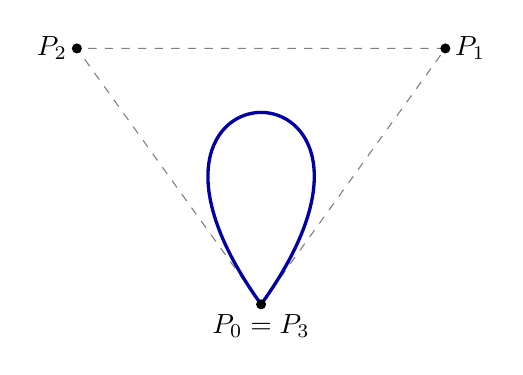
\begin{tikzpicture}[scale=1.3]
\draw[gray,dashed] (0,0)--(1.8,2.5)--(-1.8,2.5)--cycle;
\draw[blue!65!black,very thick] (0,0) .. controls (1.8,2.5) and (-1.8,2.5) .. (0,0);
\fill (0,0) circle (1.4pt) node[below] {$P_0=P_3$};
\fill (1.8,2.5) circle (1.4pt) node[right] {$P_1$};
\fill (-1.8,2.5) circle (1.4pt) node[left] {$P_2$};
\end{tikzpicture}\end{center}
\end{frame}

% Diapositiva 44
\begin{frame}[t]{Curvas de Bézier: propiedades}
Tienen un \textbf{control global}: el desplazamiento de un solo punto de control modifica la curva en todo el intervalo abierto $(0,1)$.\figura{r44_rId6.png}{.8}{.65}
\end{frame}

% Diapositiva 45
\begin{frame}[t]{Curvas de Bézier: propiedades}
Las curvas complicadas, con muchos puntos de control, se generan mediante la concatenación de varias curvas de grado menor.\figura{r45_rId6.png}{.8}{.65}
\end{frame}

% Diapositiva 46
\begin{frame}[t]{Curvas de Bézier a trozos}
Es fundamental controlar las uniones de los trozos.\figura{r46_rId4.png}{.9}{.7}
\end{frame}

% Diapositiva 47
\begin{frame}[t]{Curvas de Bézier: propiedades}
Las curvas cúbicas dan una flexibilidad razonable y evitan el incremento de cálculo producido con polinomios de grado alto.\figura{r47_rId6.png}{.85}{.63}
\end{frame}

% Diapositiva 48
\begin{frame}[t]{Curvas de Bézier: propiedades}
Se pueden crear superficies 3D a partir de curvas de Bézier.\figura{r48_rId7.png}{.85}{.68}
\end{frame}

% Diapositiva 49
\begin{frame}[t]{Curvas de Bézier: usos}
\figura{r49_rId2.png}{.95}{.82}
\end{frame}

% Diapositiva 50
\begin{frame}[t]{Curvas de Bézier: usos}
\figura{r50_rId2.png}{.95}{.82}
\end{frame}

% Diapositiva 51
\begin{frame}[t]{Curvas de Bézier: usos}
\figura{r51_rId2.png}{.95}{.82}
\end{frame}

% Diapositiva 52
\begin{frame}[t]{Curvas de Bézier: usos}
\figura{r52_rId2.png}{.95}{.82}
\end{frame}

% Diapositiva 53
\begin{frame}[t]{Curvas de Bézier: usos}
\figura{r53_rId2.png}{.95}{.82}
\end{frame}

% Diapositiva 54
\begin{frame}[t]{Curvas de Bézier: usos}
\figura{r54_rId3.png}{.95}{.82}
\end{frame}

% Diapositiva 55
\begin{frame}[t]{Superficies de Bézier}
Son superficies paramétricas cuyo dominio de parámetros es rectangular; también se denominan \textbf{parches}.\par\medskip Son una extensión directa de las curvas de Bézier. En este caso, la superficie queda parametrizada por dos variables $s$ y $t$:\[\mathbf b(s,t)=\bigl(x(s,t),y(s,t),z(s,t)\bigr),\qquad (s,t)\in[0,1]^2.\]
\end{frame}

% Diapositiva 56
\begin{frame}[t]{Superficies de Bézier: definición}
\small\[\mathbf b:[0,1]\times[0,1]\longrightarrow\mathbb R^3,\]\[\boxed{\mathbf b(s,t)=\sum_{i=0}^{m}\sum_{j=0}^{n}B_i^m(s)B_j^n(t)P_{ij}}.\]\begin{columns}[T]\begin{column}{.48\textwidth}\figura{r56_rId5.png}{1}{.46}\end{column}\begin{column}{.48\textwidth}\figura{r56_rId6.png}{1}{.46}\end{column}\end{columns}
\end{frame}

% Diapositiva 57
\begin{frame}[t]{Ejercicios}
\small\begin{enumerate}\item Dados los siguientes polígonos de control, calcular las curvas mediante polinomios de Bernstein:\begin{enumerate}\item $P_0=(0,0),\ P_1=(1,2),\ P_2=(2,-1)$.\item $P_0=(0,0),\ P_1=(1,2),\ P_2=(3,0),\ P_3=(1,-1)$.\item $P_0=(-1,0),\ P_1=(1,-1),\ P_2=(4,0),\ P_3=(2,3)$.\item $P_0=(0,0),\ P_1=(1,2),\ P_2=(2,3),$\\$P_3=(4,1),\ P_4=(3,-1)$.\end{enumerate}\item Usando los mismos ejemplos, calcular las curvas mediante el algoritmo de de Casteljau.\item ¿Qué ventajas tiene el algoritmo de de Casteljau?\item Calcular las curvas mediante su forma matricial.\end{enumerate}
\end{frame}

% Diapositiva 58
\begin{frame}[t]{Ejercicios}
\scriptsize\begin{enumerate}\setcounter{enumi}{4}\item Dados $P_0=(1,0)$, $P_1=(1,2)$ y $P_2=(3,-1)$, obtener la curva de Bézier de grado $n$ que mejor se aproxime a esos puntos.\item Calcular el paraboloide hiperbólico que pasa por $P_{00}=(0,0,0)$, $P_{01}=(0,1,1)$, $P_{10}=(1,0,1)$ y $P_{11}=(1,1,0)$.\item Calcular con de Casteljau las superficies de Bézier asociadas a las siguientes redes de control (filas: índice $i$; columnas: índice $j$):\[\begin{array}{c|ccc} &j=0&j=1&j=2\\\hline i=0&(0,0,0)&(0,1,1)&(0,2,0)\\i=1&(1,0,1)&(1,1,0)&(1,2,1)\end{array}\quad\text{bigrado }(1,2).\]\[\begin{array}{c|ccc} &j=0&j=1&j=2\\\hline i=0&(0,0,0)&(0,1,0)&(0,2,1)\\i=1&(1,0,0)&(1,1,1)&(1,2,1)\\i=2&(2,0,-1)&(2,1,0)&(2,2,0)\end{array}\quad\text{bigrado }(2,2).\]\item Repetir el ejercicio anterior usando los polinomios de Bernstein.\end{enumerate}
\end{frame}
\end{document}
